\chapter{Initial Data Analysis}\label{Sec:Initial Data Analysis}

In order to diagnose to what extent an algorithm suffers from sampling bias, it will be useful to have another dataset. Initial data analysis is conducted independently of the problem statements to understand what properties of the data differ between GBS and GESIS for matching attributes. A brief characterization of the data currently employed in the studies is given in this chapter. The GitHub repository further specifies the list of transformations that are sequentially applied to each group of features in order to prepare the inputs for survey comparisons. Preprocessing steps and methods used to evaluate outcomes are documented as well. Scaling methods that apply to both data sets, e.g: centering and scaling of skewed continuous features for SVMs, are not mentioned but can be deduced from code easily. If an attribute is removed at some point, it will only be mentioned in the relevant section.

\begin{figure}[ht]
	\begin{center}
		\captionsetup{width= 425pt}
		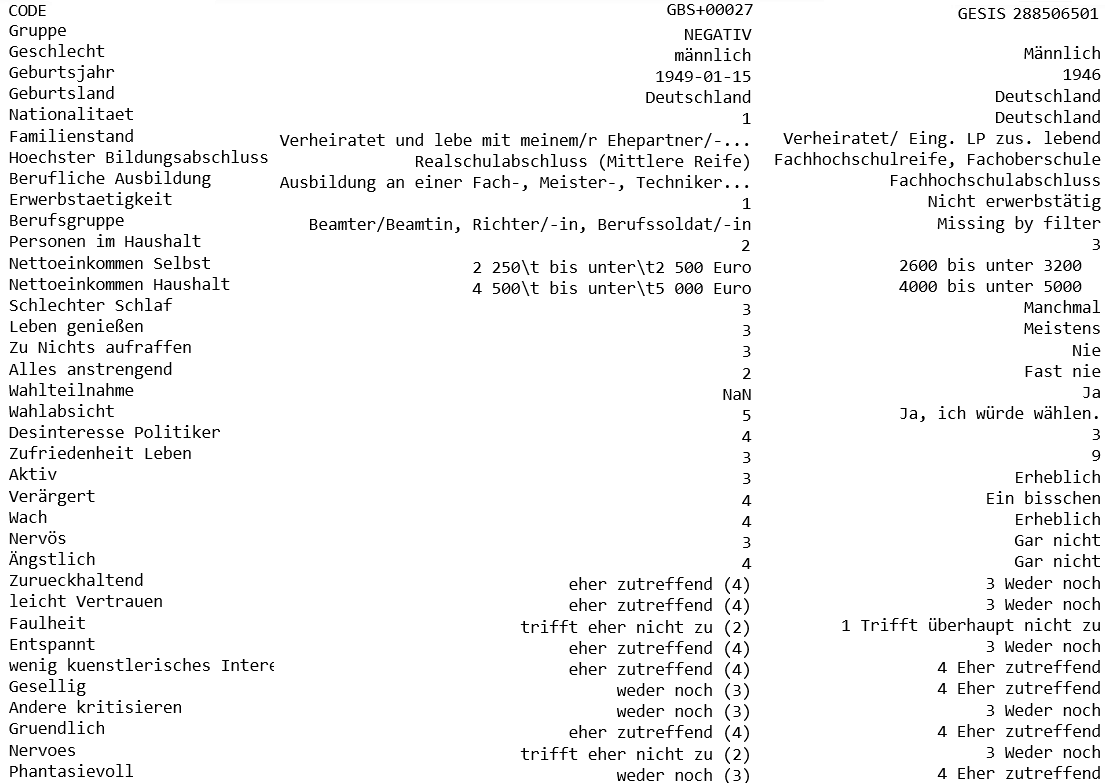
\includegraphics[scale=0.52,angle=0]{fig/values_compare}
		\label{std}
		\caption{GBS - GESIS attribute and value comparison. Not all attributes are used in every learning task. See GitHub documentation for more information.}
	\end{center}
\end{figure}

\section{Feature Selection and Data Imputation}

If not stated differently, deletion of rows is applied to every instance with missing values in GESIS to reduce the class imbalance in the later described classification problem. Missing values are sparse in GBS and can be imputed, e.g: with median substitution, with negligible effects. Mean substitution can not be used as this might lead to previously unseen values. Discriminative algorithms will then use these new values to distinguish GBS and GESIS that have been created by ill-considered data imputation. Note that the following figures represent the data after attribute and value matching described in Sec. 2.2.

Fig. A.2 lends itself to first thoughts about whether missing data elements depend on observable attributes or occur entirely at random and is also able to detect functional dependencies in GESIS. Fig. A.3 summarizes the main observations from GBS. The correlation matrix with ratio -1 to +1 in Fig. A.4 is used as another way to visualize differences in GESIS and GBS and to further simplify preprocessing decisions. Potential bugs and issues can also be detected with this graph. 

\begin{figure}[h]
	\begin{center}
		\captionsetup{width= 400pt}
		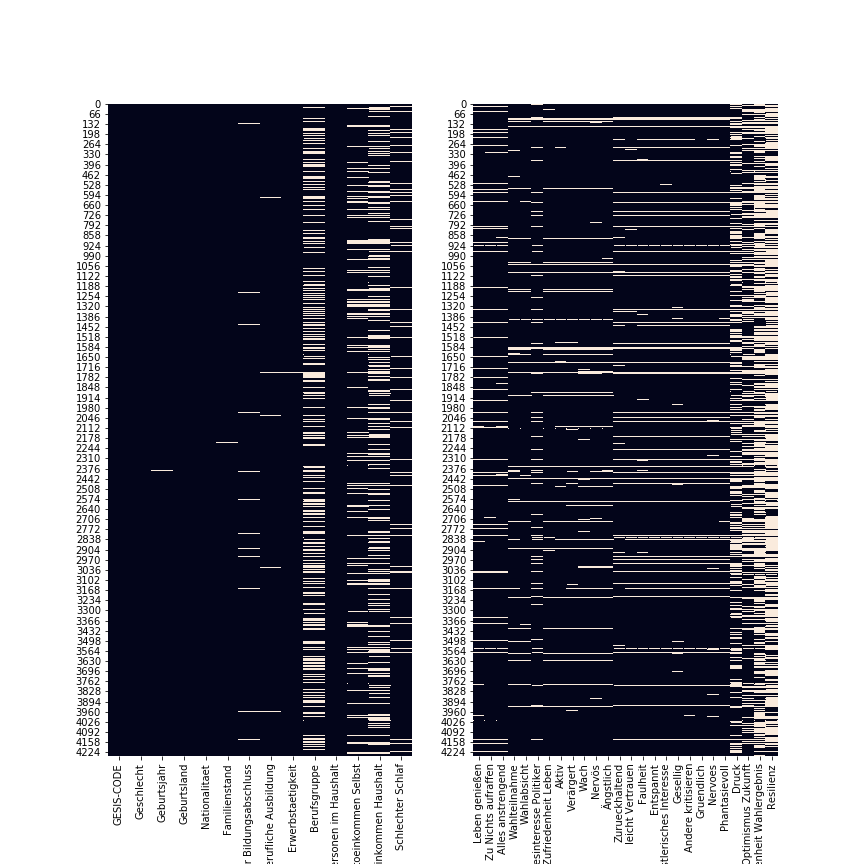
\includegraphics[scale=0.50,angle=0]{fig/gesis_missing}
		\label{gesis_miss}
		\caption{Missing values in GESIS. The attribute values of a participant are always known for "Geschlecht", "Geburtsland", "Geburtsjahr", "Nationalitaet", "Familienstand", "Personen im Haushalt". In contrast, the last three columns "Druck", "Optimismus Zukunft", "Zufriedenheit Wahlergebnisse" and "Resilienz" are almost always missing and are therefore removed from the analysis. Participants with missing BFI-10 elements are removed. Sample size will only be reduced slightly as missing values often occur for the same instance. These dependencies form a line pattern in the graph. "Berufsgruppe" was surveyed as a text field so that the column clearly suffers from ambiguous value mismatch. To include "Berufsgruppe" mappings need to be redefined first. For now, "Berufsgruppe" is removed. }
	\end{center}
\end{figure}

\begin{figure}[ht]
	\begin{center}
		\captionsetup{width= 400pt}
		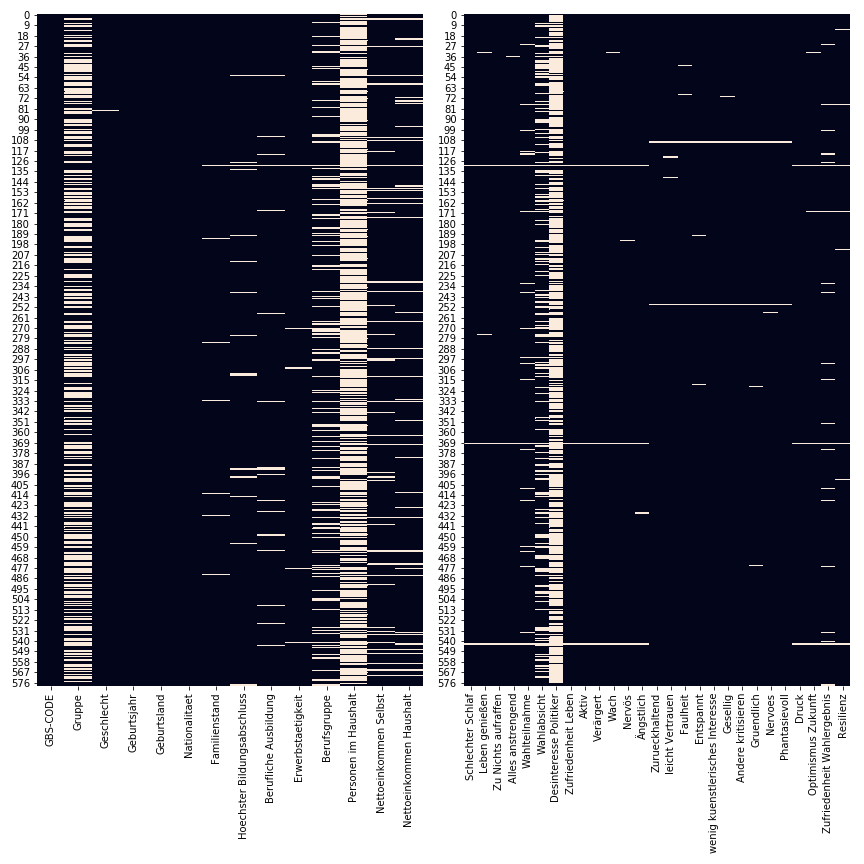
\includegraphics[scale=0.50,angle=0]{fig/gbs_missing}
		\label{gbs_miss}
		\caption{Missing values in GBS. There is one more attribute in "Gruppe". Not every participant received a positive a negative psychological treatment. Therefore, "Gruppe" is more likely to be missing than not. However, the absence of a value indicates no treatment rather than a missing positive or negative. "Gruppe" is not properly represented yet. "Desinteresse Politiker" is given by multiple data sources from different excel files. Some of them being the inverse of the attribute itself. The surey design regarding this issue is unclear to me. To incorporate "Desinteresse Politiker" the attribute(s) need to be imported correctly, if possible. Another import issue is given by "Personen im Haushalt". If the actual value is greater than one, the cell will be empty. To correct this, the corresponding csv-file needs to be fixed. The text field "Berufsgruppe" suffers on both ends, GBS and GESIS, due to current oversimplification of value and potential data mismatch.}
	\end{center}
\end{figure}

\begin{figure}[ht]
	\begin{center}
		\captionsetup{width= 400pt}
		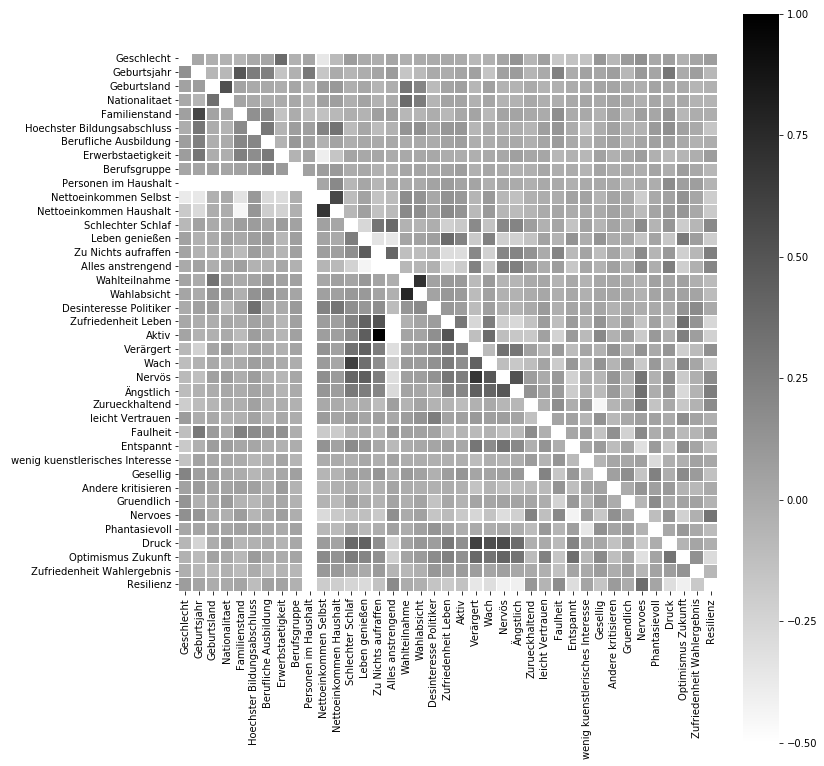
\includegraphics[scale=0.73,angle=0]{fig/correl}
		\label{corr}
		\caption{The upper right triangular matrix shows GESIS correlations while GBS correlations are shown in the lower left. The main diagonal should not be confused with white squares. These trivial combinations are simply excluded and not colored black. As can be seen "Personen im Haushalt" in GBS can not be calculated, since there is only one possible value. "Nettoeinkommen Selbst" and "Nettoeinkommen Haushalt" are highly correlated but not removed or handled at all. I will keep this in mind, when facing the naive bayes assumption in the learning process. Entropy-based mutual information in "Wahlteilnahme" and "Wahlabsicht" have led to almost perfect classification performances in predicting political participation. "Wahlabsicht" is therefore removed.}
	\end{center}
\end{figure}

\section{Perspectives on Response Styles}

In survey analysis, scales measuring attributes need to be reliable and valid. Therefore, GBS and GESIS almost entirely use already tested scales from the literature. Although the same characteristics are asked in both surveys, they may have been covered differently, for example by different scales. In addition, GBS surveys are generally more detailed. Especially characteristics which are not exactly predefined are often recorded differently. Features must be engineered carefully, whereby potential loss of information must be minimized. Shortcomings in attribute mappings may result in inappropriate representation and therefore incorrect conclusions. The Big Five are a consistent set of attributes across the surveys. In contrast, there also exist vivid examples for data mismatch on Likert-type scales.

\subsection{Likert-Type Scale}

The Big Five is an empirically-derived model of human personality and psyche. When factor analysis is applied to personality survey data, five clusters of traits consistently emerge. The BFI-10 is a 10-item scale measuring the Big Five personality traits. Figures 2.5 visualizes the response distribution of two BFI items for the "Conscientiousness" dimension, representing both the high and low pole. "Agreeableness", "Extraversion", "Neuroticism" and "Openness" can be compared in the output folder of the project repository \cite{rammstedt}. 

Likert scales are the most frequently used instruments in GBS and GESIS. They consist of statements which measure the intensity of one's estimation towards the preceding statement. Respondents are asked to rate the BFI-10 items on a level of agreement on a consistent rating scale ranging from "Strongly Agree (5)" to Strongly Disagree (1)" for all items in both surveys \cite{likert}. 

\begin{figure}[H]
	\begin{center}
		\captionsetup{width= 380pt}
		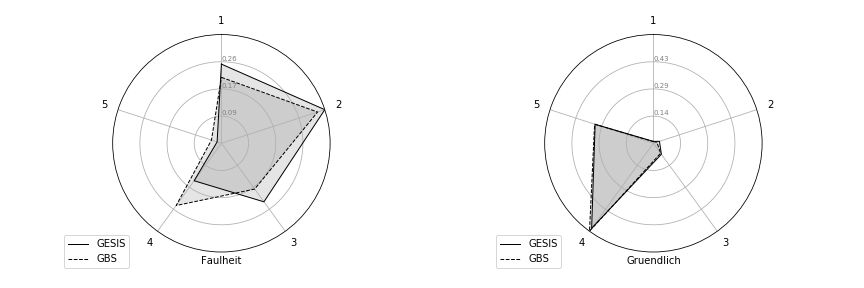
\includegraphics[scale=0.48,angle=0]{fig/Conscientiousness_figure}
		\label{Conscientiousness}
		\caption{Conscientiousness is the degree of organization, self-regulation, and responsibility one exhibits. \textit{"I see myself as someone who tends to be lazy."}(left). \textit{"I see myself as someone who does a thorough job."}(right). The graphs are almost identical for the Likert item "Gruendlich". Respondents specify their level of disagreement for "Faulheit" stronger in GBS.}
	\end{center}
\end{figure}

There are still discussions about whether to use a Likert scale element as a categorical or numerical characteristic. The intervals between positions on the scale are monotonous, but never so well defined that they are numerically uniform steps. A "Strongly Agree (5)" answer indicates more agreement than "Agree", but it shows no agreement that is five times stronger than "Strongly Disagree (1)". In this work, the BFI-10 items are considered categorical, considering the use and limitations of Likert scales \cite{likert2, likert3}.

\subsection{Data Mismatch}

\begin{table}[ht]
    \begin{center}
	\captionsetup{width= 400pt}
            {\footnotesize
            \begin{tabular}{l|c|ccccccccc}
                \hline \hline
		attribute & GBS values & GBS values count &  GESIS values & GESIS values count \\
                \hline \hline
                     Wach & 4 & 311 & Einigermassen & 1697 \\
                     & 3 & 183 & Erheblich & 1389 \\
                     & 2 & 66 & Ein bisschen & 467 \\ 
              	& 1 & 14 & Aeusserst & 367 \\	
		& -1 & 1 & Gar nicht & 184 \\		
	     \hline \hline
            \end{tabular}}
        \caption{"Wach" as an example of a Likert item discrepancy. GESIS uses an odd number of responses with a "neutral" option, such as "no opinion", "neither agree nor disagree" or some phrase to that effect. In contrast, there is an even number of responses for this item in GBS encouraging participants to voice a positive or negative opinion. In some cases, an additional "opt-out" option is provided for those respondents who truly cannot respond. The respondent may not respond because some questions are too sensitive. This type of nonresponse would also be considered missing values indicated by "-1" \cite{likert4}.}
\end{center}
\end{table}

It can be assumed that different numbers of rating bars in a subjective rating scale can have significant effects on the subjective measurement \cite{heeringa}. Table 2.1 gives an example for two different scales of the same attribute while trying to find a proper representation in Table 2.2. GESIS often contains textual values, which often cannot be clearly assigned to numeric scales, so that the value counts have to be used to support the decision making. Figure 2.7 shows what happens when attributes are partially transformed using cut-off mappings. MAYBE PUT ANOTHER SENTENCE HERE JUST SO THAT IT LOOKS BETTER. A SECOND SENTENCE WOULD LOOK EVEN BETTER OKAY??

\vspace{0.48cm}
\begin{table}[ht]
    \begin{center}
	\captionsetup{width= 400pt}
            {\footnotesize
            \begin{tabular}{l|c|ccccccccc}
                \hline \hline
		Raw Data & GESIS & 1 & 2 & 3 & 4 & 5 & 6 \\
                     & GBS & 1 & 2 & 3 & 4 & 5 & \\
                \hline
		Max Scaler & GESIS & 0.83 & 1.7 & 2.5 & 3.3 & 4.2 & 5.0 \\
                     & GBS & 1 & 2 & 3 & 4 & 5 & \\
                \hline
		Min-Max Scaler & GESIS & 1 & 1.8 & 2.6 & 3.4 & 4.2 & 5 \\
                     & GBS & 1.0 & 2.25 & 3.5 & 4.75 & 6.0 & \\
                \hline
		Cut-Off Mapping & GESIS & 1 & 2 & 3 & 4 & 5 & 5 \\
                     & GBS & 1 & 2 & 3 & 4 & 5 & \\
	     \hline \hline
            \end{tabular}}
        \caption{Demonstration of potential scalings for differing attribute values. The cut-off mapping comes with a loss of information. Max scaler and min-max scaler introduce new unseen values that can be problematic for statistical learning.}
\label{Tab:DescripStatsRawData}
\end{center}
\end{table}

\begin{figure}[ht]
	\begin{center}
		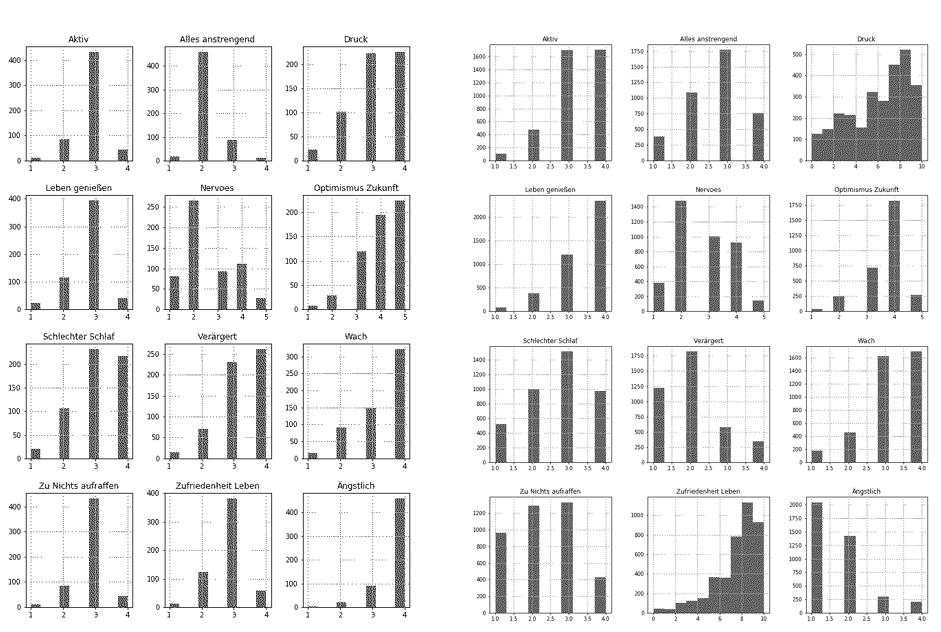
\includegraphics[scale=0.62,angle=0]{fig/histo}
		\label{std}
		\caption{Overview of attributes that can not be used for further analysis due to data mismatch. GESIS histograms (right) are show differently scaled values, some of which have been transformed already. Taking the inverse of "Aengstlich", "Alles anstrengend" and perhaps "Veraergert" for either the left or right side is likely to match the values properly. The remaining attributes do not seem to be reliable and will not be included for the time being. Depending on the discriminative algorithm, values ​​that only appear in one of the two surveys are enough to perfectly classify instances: "\textit{If value equals 1.7  \(\rightarrow\) Instance of class GESIS}". Decision-tree based learning algorithms will likely suffer from erroneous mappings, while logistic regression with a proper scoring rule might be the most suitable algorithm to limit the effects of measurement discrepancy.}
	\end{center}
\end{figure}



